\documentclass{article}
\usepackage[utf8]{inputenc}
\usepackage{graphicx}
\usepackage[pdftex]{hyperref}

\title{Circuitos digitais}
\author{Amanda Aparcida Machado Goulart - 133569 }
\date{Setembro 2020}

\begin{document}

\maketitle

\section{Laboratório 01}
\subsection{Objetivo}
Implemente um circuito digital que simule um jogo de dois dados entre dois jogadores.
\\
Cada jogador lançará agora um par de dados e aquele que obtiver a maior soma dos valores é o
vencedor.
\\
Como entrada, o circuito possui quatro sinais com 3 entradas, sendo 2 para cada jogador representando
valores entre 1 e 6 que cada jogador tirou no seu par de dados.
Dados os valores das somas dos dados, o jogo deve gerar como saída um de três sinais que indicará a
vitória do jogador 1, a vitória do jogador 2 ou um empate. O jogador com a maior soma vence.
\\
Essa versão do jogo deve ter também um placar composto por dois displays de 7 segmentos para cada
jogador indicando a soma que obteve ao lançar os seus dados.
Use switches para os sinais de entrada e leds para as saídas indicando o jogador vencedor ou empate.
\\
Não precisa sortear os valores. Considere que as entradas são dadas apenas para verificar o resultado do
jogo.

\subsection{Implementação para verificar ganhador}

\begin{figure}[!h]
\centering
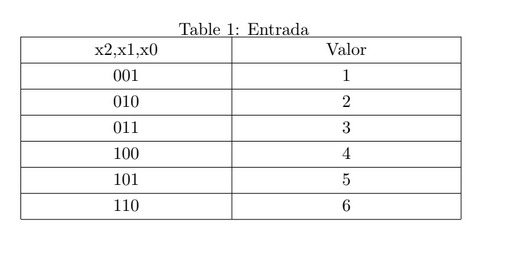
\includegraphics[width=5cm]{img01.jpeg}
\caption{Lógica para implementação 01}
\label{fig:CL_logo}
\end{figure}

\subsubsection{Mapa de Karnaugh}

Primeiramente para fazer a conversão de binário para Grey foi feita o seguinte mapa da karnaugh.

\begin{figure}[!h]
\centering
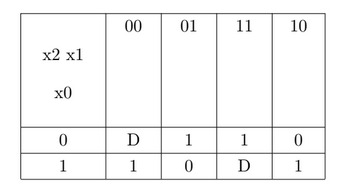
\includegraphics[width=5cm]{img02.jpeg}
\caption{Karnaught para y0}
\label{fig:CL_logo}
\end{figure}

Com a equação: (x1 !x0)+(!x1 x0)

\begin{figure}[!h]
\centering
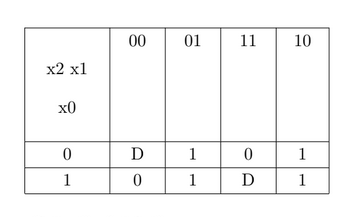
\includegraphics[width=5cm]{fig03.png}
\caption{Karnaught para y1}
\label{fig:CL_logo}
\end{figure}

Resultando em: (!x2 x1)+(x2 !x1)

\begin{figure}[!h]
\centering
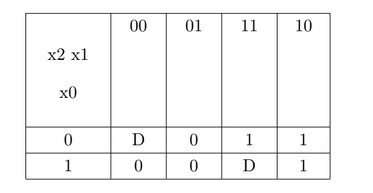
\includegraphics[width=5cm]{fig04.png}
\caption{Karnaught para y2}
\label{fig:CL_logo}
\end{figure}

Resultando em: (x2 !x0)+(x2 !x1)
\\
\\
\\
\\
Posteriomente foi feita uma comparação para verificar se são identicos.
\\
\\
\\
\\

\begin{figure}[!h]
\centering
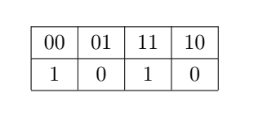
\includegraphics[width=5cm]{fig05.png}
\caption{Comparação}
\label{fig:CL_logo}
\end{figure}


Resultando em (\overline{xi}∙\overline{yi})+(xi∙yi) = xi \oplus yi

Para verificar se é maior ou menor:

\begin{figure}[!h]
\centering
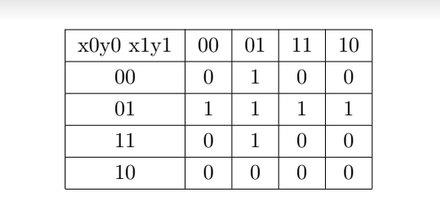
\includegraphics[width=5cm]{fig06.png}
\caption{Karnaught para x2}
\label{fig:CL_logo}
\end{figure}

Agora avaliando para x1, x2, y1, y2:

Para y2:
\begin{figure}[!h]
\centering
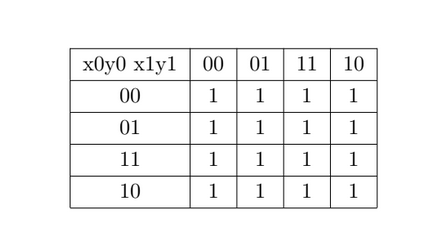
\includegraphics[width=5cm]{fig07.png}
\caption{Karnaught para y2}
\label{fig:CL_logo}
\end{figure}

Para x1:

\begin{figure}[!h]
\centering
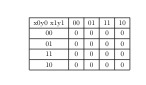
\includegraphics[width=5cm]{x1.jpeg}
\caption{Karnaught para x1}
\label{fig:CL_logo}
\end{figure}

Para y1:

\begin{figure}[!h]
\centering
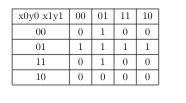
\includegraphics[width=5cm]{y1.jpeg}
\caption{Karnaught para y1}
\label{fig:CL_logo}
\end{figure}

Resultando em: (\overline{x2}∙y2)+(\overline{x2}∙\overline{x1}∙y1)+(\overline{x2}∙\overline{x1}∙\overline{x0}∙y0)+(x2∙y1∙\overline{x0}∙y0)+(y2∙\overline{x1}∙y1)+(y2∙\overline{x1}∙\overline{x0}∙y0)+(y2∙y1∙\overline{x0}∙y0)

\subsection{Circuito}
\begin{figure}[!h]
\centering
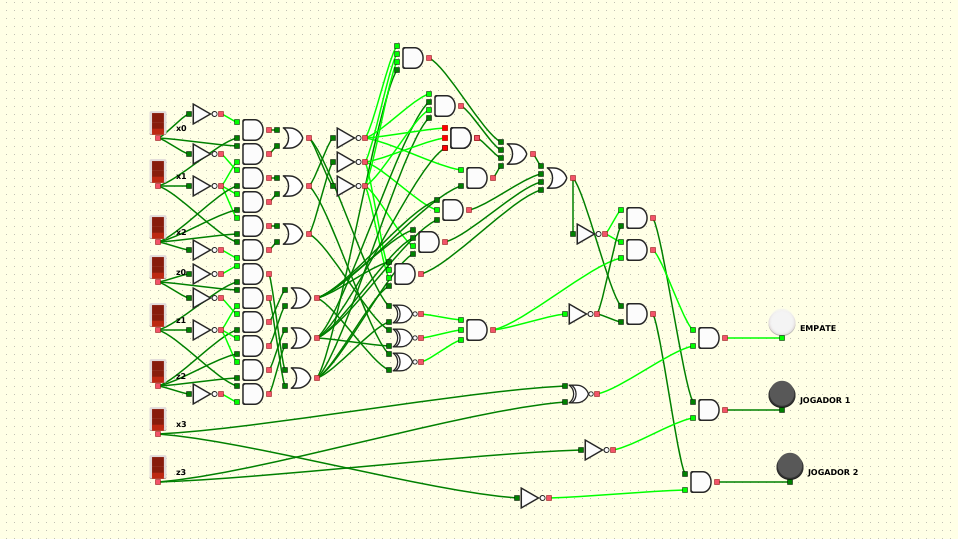
\includegraphics[width=15cm]{c1.png}
\caption{Circuito para saber qual vencedor}
\label{fig:CL_logo}
\end{figure}

\subsection{Implementação para soma de 2 bits}

\begin{figure}[!h]
\centering
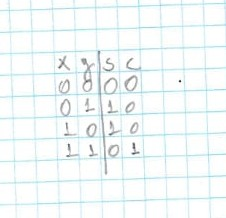
\includegraphics[width=3cm]{somaSimples.jpeg}
\caption{Lógica soma de dois bits}
\label{fig:CL_logo}
\end{figure}

s=x⊕y;
\\
c=x∙y

\subsection{Circuito}
\begin{figure}[!h]
\centering
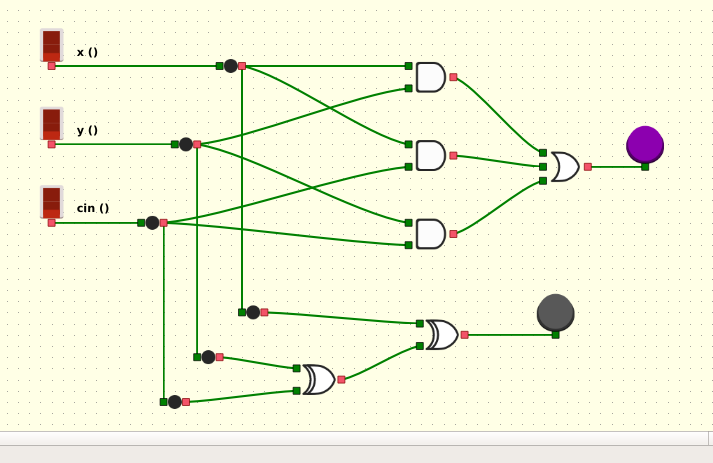
\includegraphics[width=15cm]{c2.png}
\caption{circuito soma de dois bits}
\label{fig:CL_logo}
\end{figure}

\subsection{Implementação para soma aninhada}

\begin{figure}[!h]
\centering
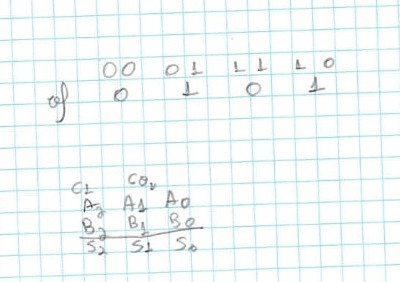
\includegraphics[width=5cm]{somaAninhada.jpeg}
\caption{Lógica de soma aninhada}
\label{fig:CL_logo}
\end{figure}

\subsection{Circuito}
\begin{figure}[!h]
\centering
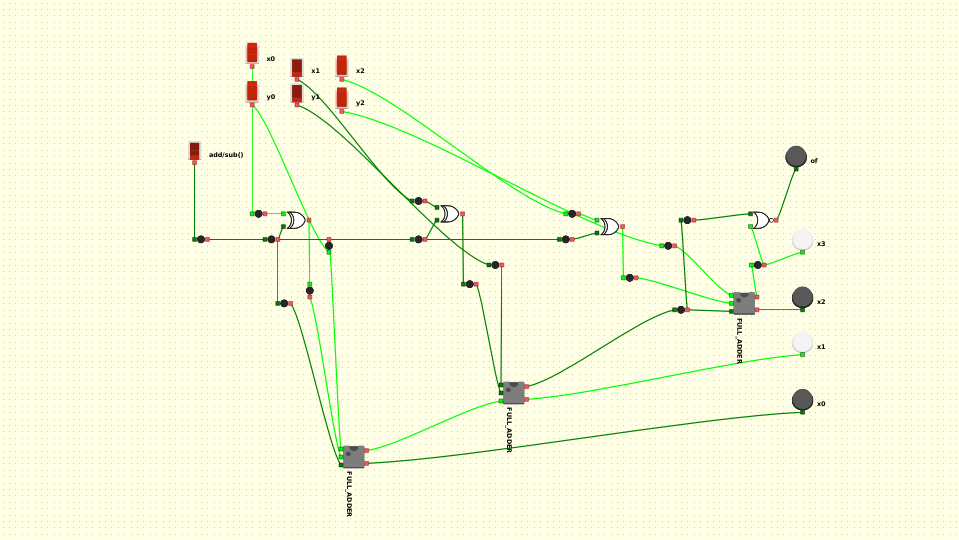
\includegraphics[width=15cm]{c3.png}
\caption{Circuito de soma aninhada}
\label{fig:CL_logo}
\end{figure}

\subsection{Implementação para display}
\begin{figure}[!h]
\centering
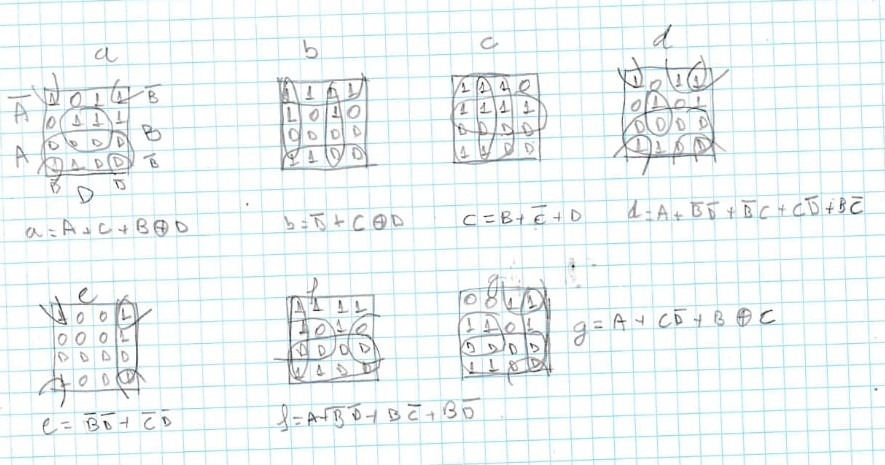
\includegraphics[width=15cm]{k.jpeg}
\caption{Mapa de Karnaugh para o display}
\label{fig:CL_logo}
\end{figure}

\subsection{Circuito finalizado}

\subsection{Implementação para display}
\begin{figure}[!h]
\centering
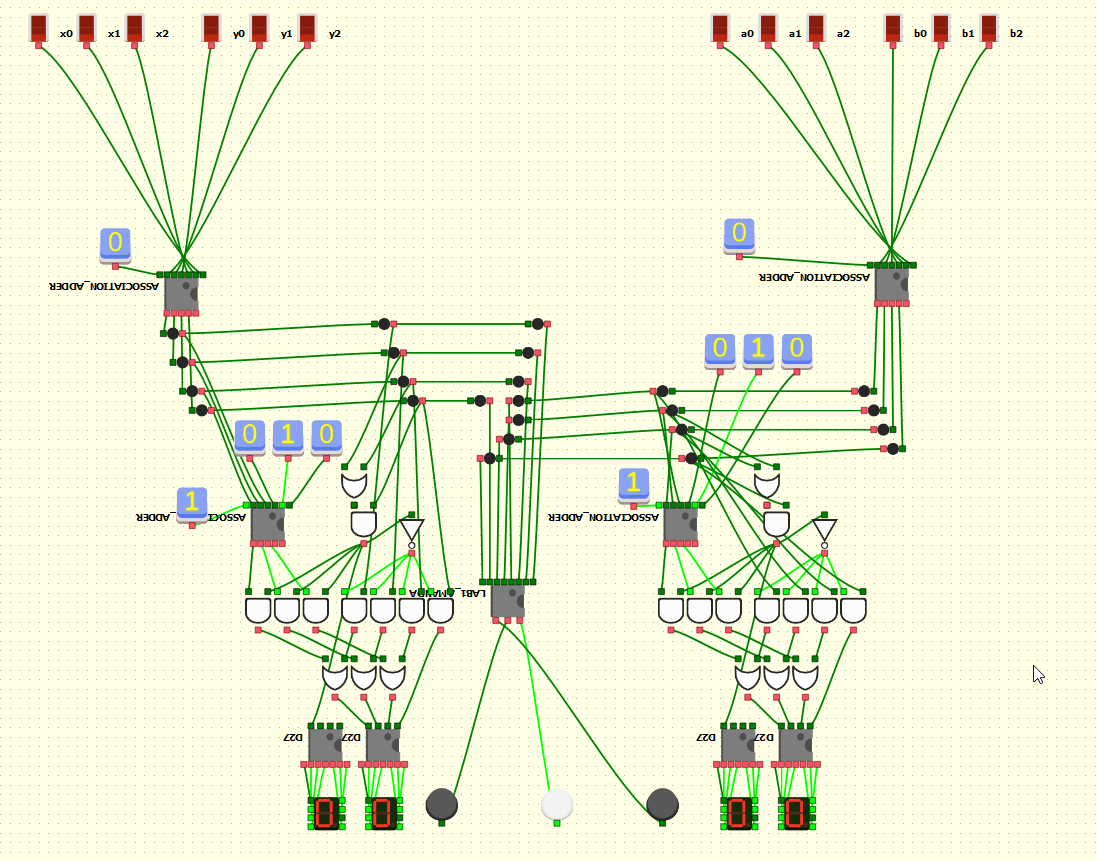
\includegraphics[width=15cm]{c4.png}
\caption{Mapa de Karnaugh para o display}
\label{fig:CL_logo}
\end{figure}



\end{document}